\chapter{Algorithms}
\label{ch:algorithms}



\section{Intuition}
\label{sec:intuition}

To solve this problem we have to evaluate all possible edge combinations. Even for greedy heuristics we need to limit the edge candidates. The algorithm considers nodes with a high expressed value. According to our model the smallest decrease is happening when we connect a value near zero and a relatively high value.
\\
\\
We will now see why this statement holds by examining how the expressed opinion changes with an addition in the Friedkin and Johnsen model. Consider an arbitrary example with two nodes inside a network. Node $a$ has $z_a = -0.02$ and node $b$ has $z_b = 0.5$. Also for this example we assume that $w_{ii}=w_{ij}=w_{ji}=1$. 
\\
\\
If we connect these two nodes with an edge and re calculate the expressed opinions both of the $z_i$ denominators will be increased by one. This emerges from the fact that both nodes will have an additional neighbour and that all weights equal with one. The numerator of the one node $a$ will be increased by a lot and the numerator of the node $b$ will be decreased by a small value.
\\
\\
The new $z_a$ will not change a lot because the big addition in the numerator will approach the +1 addition of the denominator. On the other hand the new $z_b$ will see a big change as the numerator had a small decrease thus creating a big decrease overall for this node. We can clearly see that only one of the two nodes will amount to a big decrease. 
\\
\\
Now consider a second example of two nodes node $c$ has $z_c = -0.8$ and node $d$ has $z_d = 0.9$. After the addition node $d$ will see a big decrease because we add two conflicting values that almost neutralise each other on the numerator but the addition of the +1 on the denominator stands still. On the other hand node $c$ will also see a big decrease for the same reason. With this type of connection both of the nodes have a significant decrease.
\\
\section{Properties of nodes having  large decrease}
\label{sec:properties}

When analysing a social graph we need centrality measures. We will examine nodes that have a large decrease of the polarization index in contrast with nodes that the decrease is almost insignificant. 
One of the centrality measures is the betweenness centrality. This metric measures the number of times a node lies on the shortest path between other nodes and shows which nodes are bridges between nodes in a network. 
Another metric is the closeness centrality. This metric scores each node based on their closeness to all other nodes in the network by calculating the shortest paths between all nodes and assigning each node a score based on its sum of shortest paths. 
Finally eigen centrality will measure a node's influence based on the number of links it has but also taking into account how well connected a node is, and how many links their connections have.
\\
\\
The karate club social network\cite{nr} consists of a small pollarized community between two opposing karate teachers and their followers. After finding all possible connections between opposing opinions we compare the betweenness, closeness and Eigen centrality of them.
\\
\\

\begin{table}[t]
 \centering
 \caption{Nodes with the 5 largest decrease}
 \label{tab:nodesLargest}
 \begin{tabular}{| l || l | l | l |}
 \hline
  Node id & Closeness Centrality& Betweeness Centrality & Eigen Centrality\\
  \hline
  \hline
  6 & 0.38372 & 0.02998 & 0.07948\\
  \hline
  7 & 0.38372 & 0.02998 & 0.07948\\
  \hline
  17 & 0.28448 & 0.0 &  0.02363\\
  \hline
  26 & 0.375 & 0.00384 & 0.05920\\
  \hline
  30 & 0.38372 & 0.00292 & 0.13496\\
  \hline
  \hline
  Norm & 0.814420 & 0.042682 & 0.186853\\ 
  \hline
 \end{tabular}
\end{table}



\begin{table}[t]
 \centering
 \caption{Nodes with the 5 smallest decrease}
 \label{tab:nodesSmallest}
 \begin{tabular}{| l || l | l | l |}
 \hline
  Node id & Closeness Centrality& Betweeness Centrality & Eigen Centrality\\
  \hline
  \hline
  3 & 0.55932 & 0.143656 & 0.31718\\
  \hline
  9 & 0.51562 & 0.05592 & 0.22740\\
  \hline
  10 & 0.43421 & 0.00084 &  0.10267\\
  \hline
  31 & 0.458333 & 0.01441 & 0.17476\\
  \hline
  33 & 0.51562 & 0.14524 & 0.30865\\
  \hline
  \hline
    Norm & 1.11498 & 0.21229 & 0.53728\\ 
  \hline
 \end{tabular}
\end{table}


Nodes with the smallest decrease of polarization index have bigger betweenness, closeness and Eigen centrality. This means that these nodes are individuals who influence and are better placed to influence the flow around the whole network. This leads us to consider connecting nodes that not only have high opposing opinions but also lie in the periphery of the network and are more isolated. 
\\
\\
These additions can be seen in figures ~\ref{fig:largest} and ~\ref{fig:smalest} of the karate  network graph. Central nodes are bigger, polarized nodes with a value of $+1$ have a red color and nodes with a value of $-1$ have a blue colour.


\begin{figure}[!htb]
	\centering
 	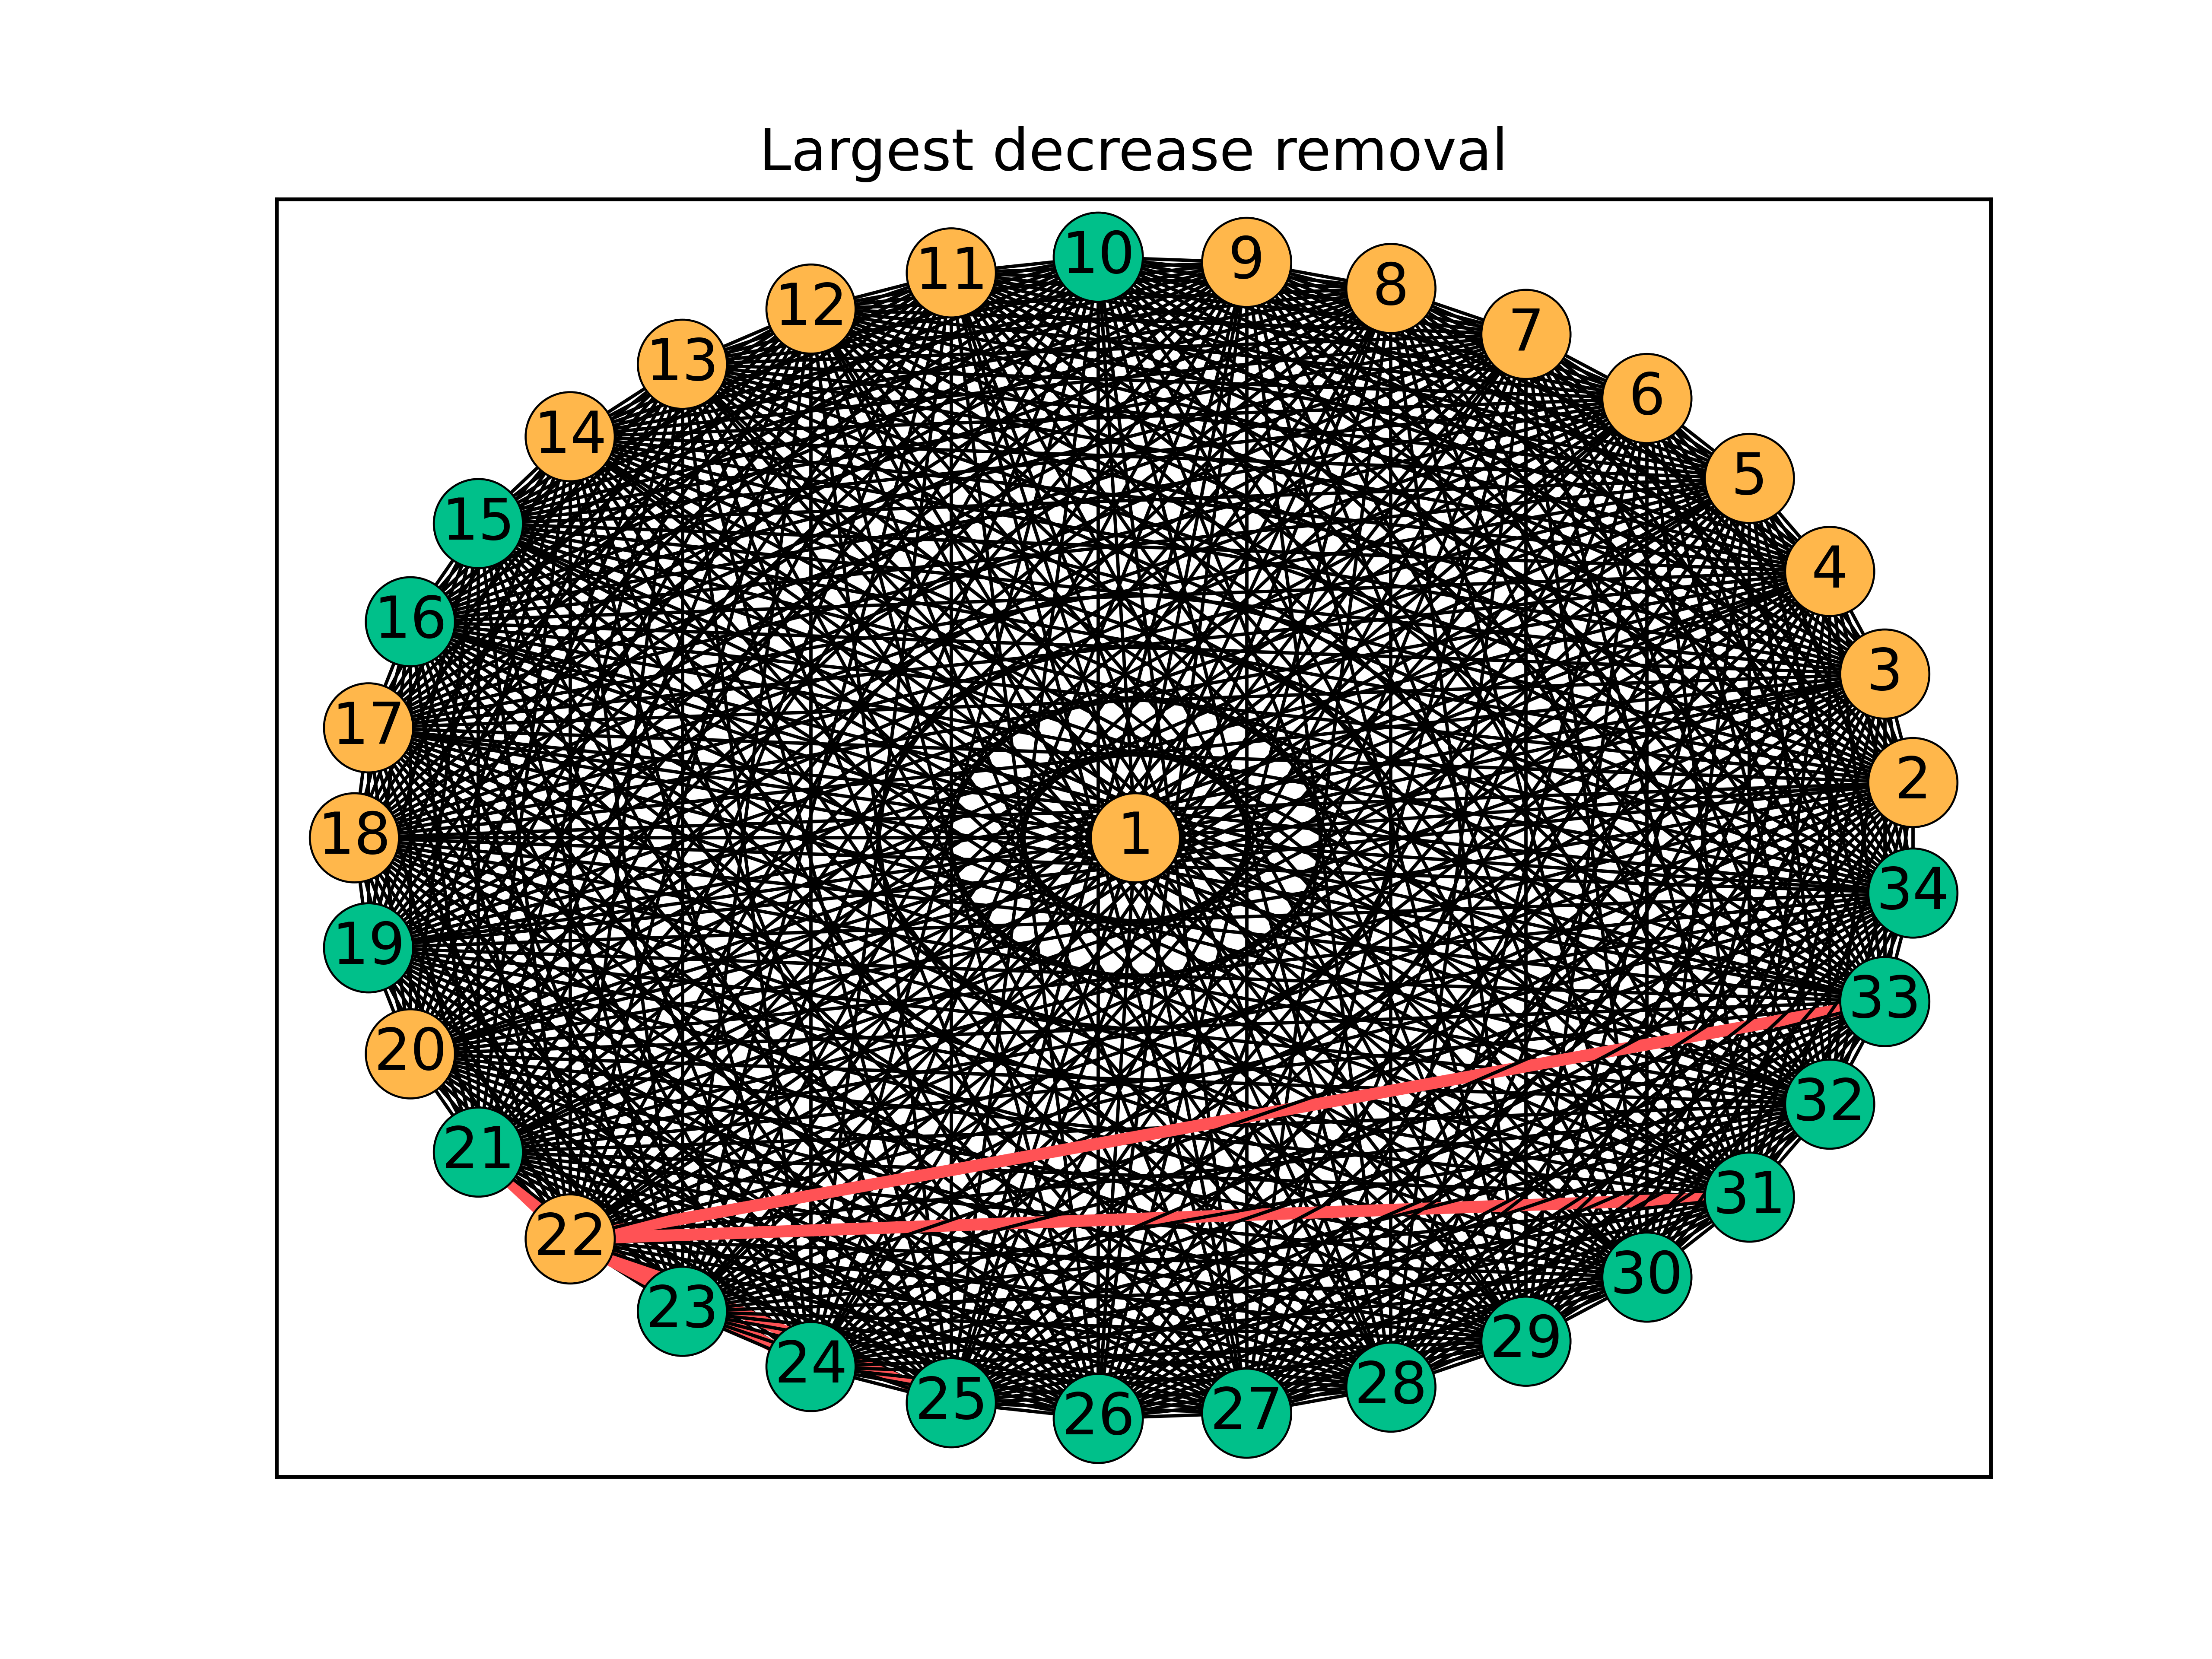
\includegraphics[width=0.70\textwidth]{Figures/largest.png}
	\caption{Edge additions}
 	\label{fig:largest}
	
	\vspace{\floatsep}
	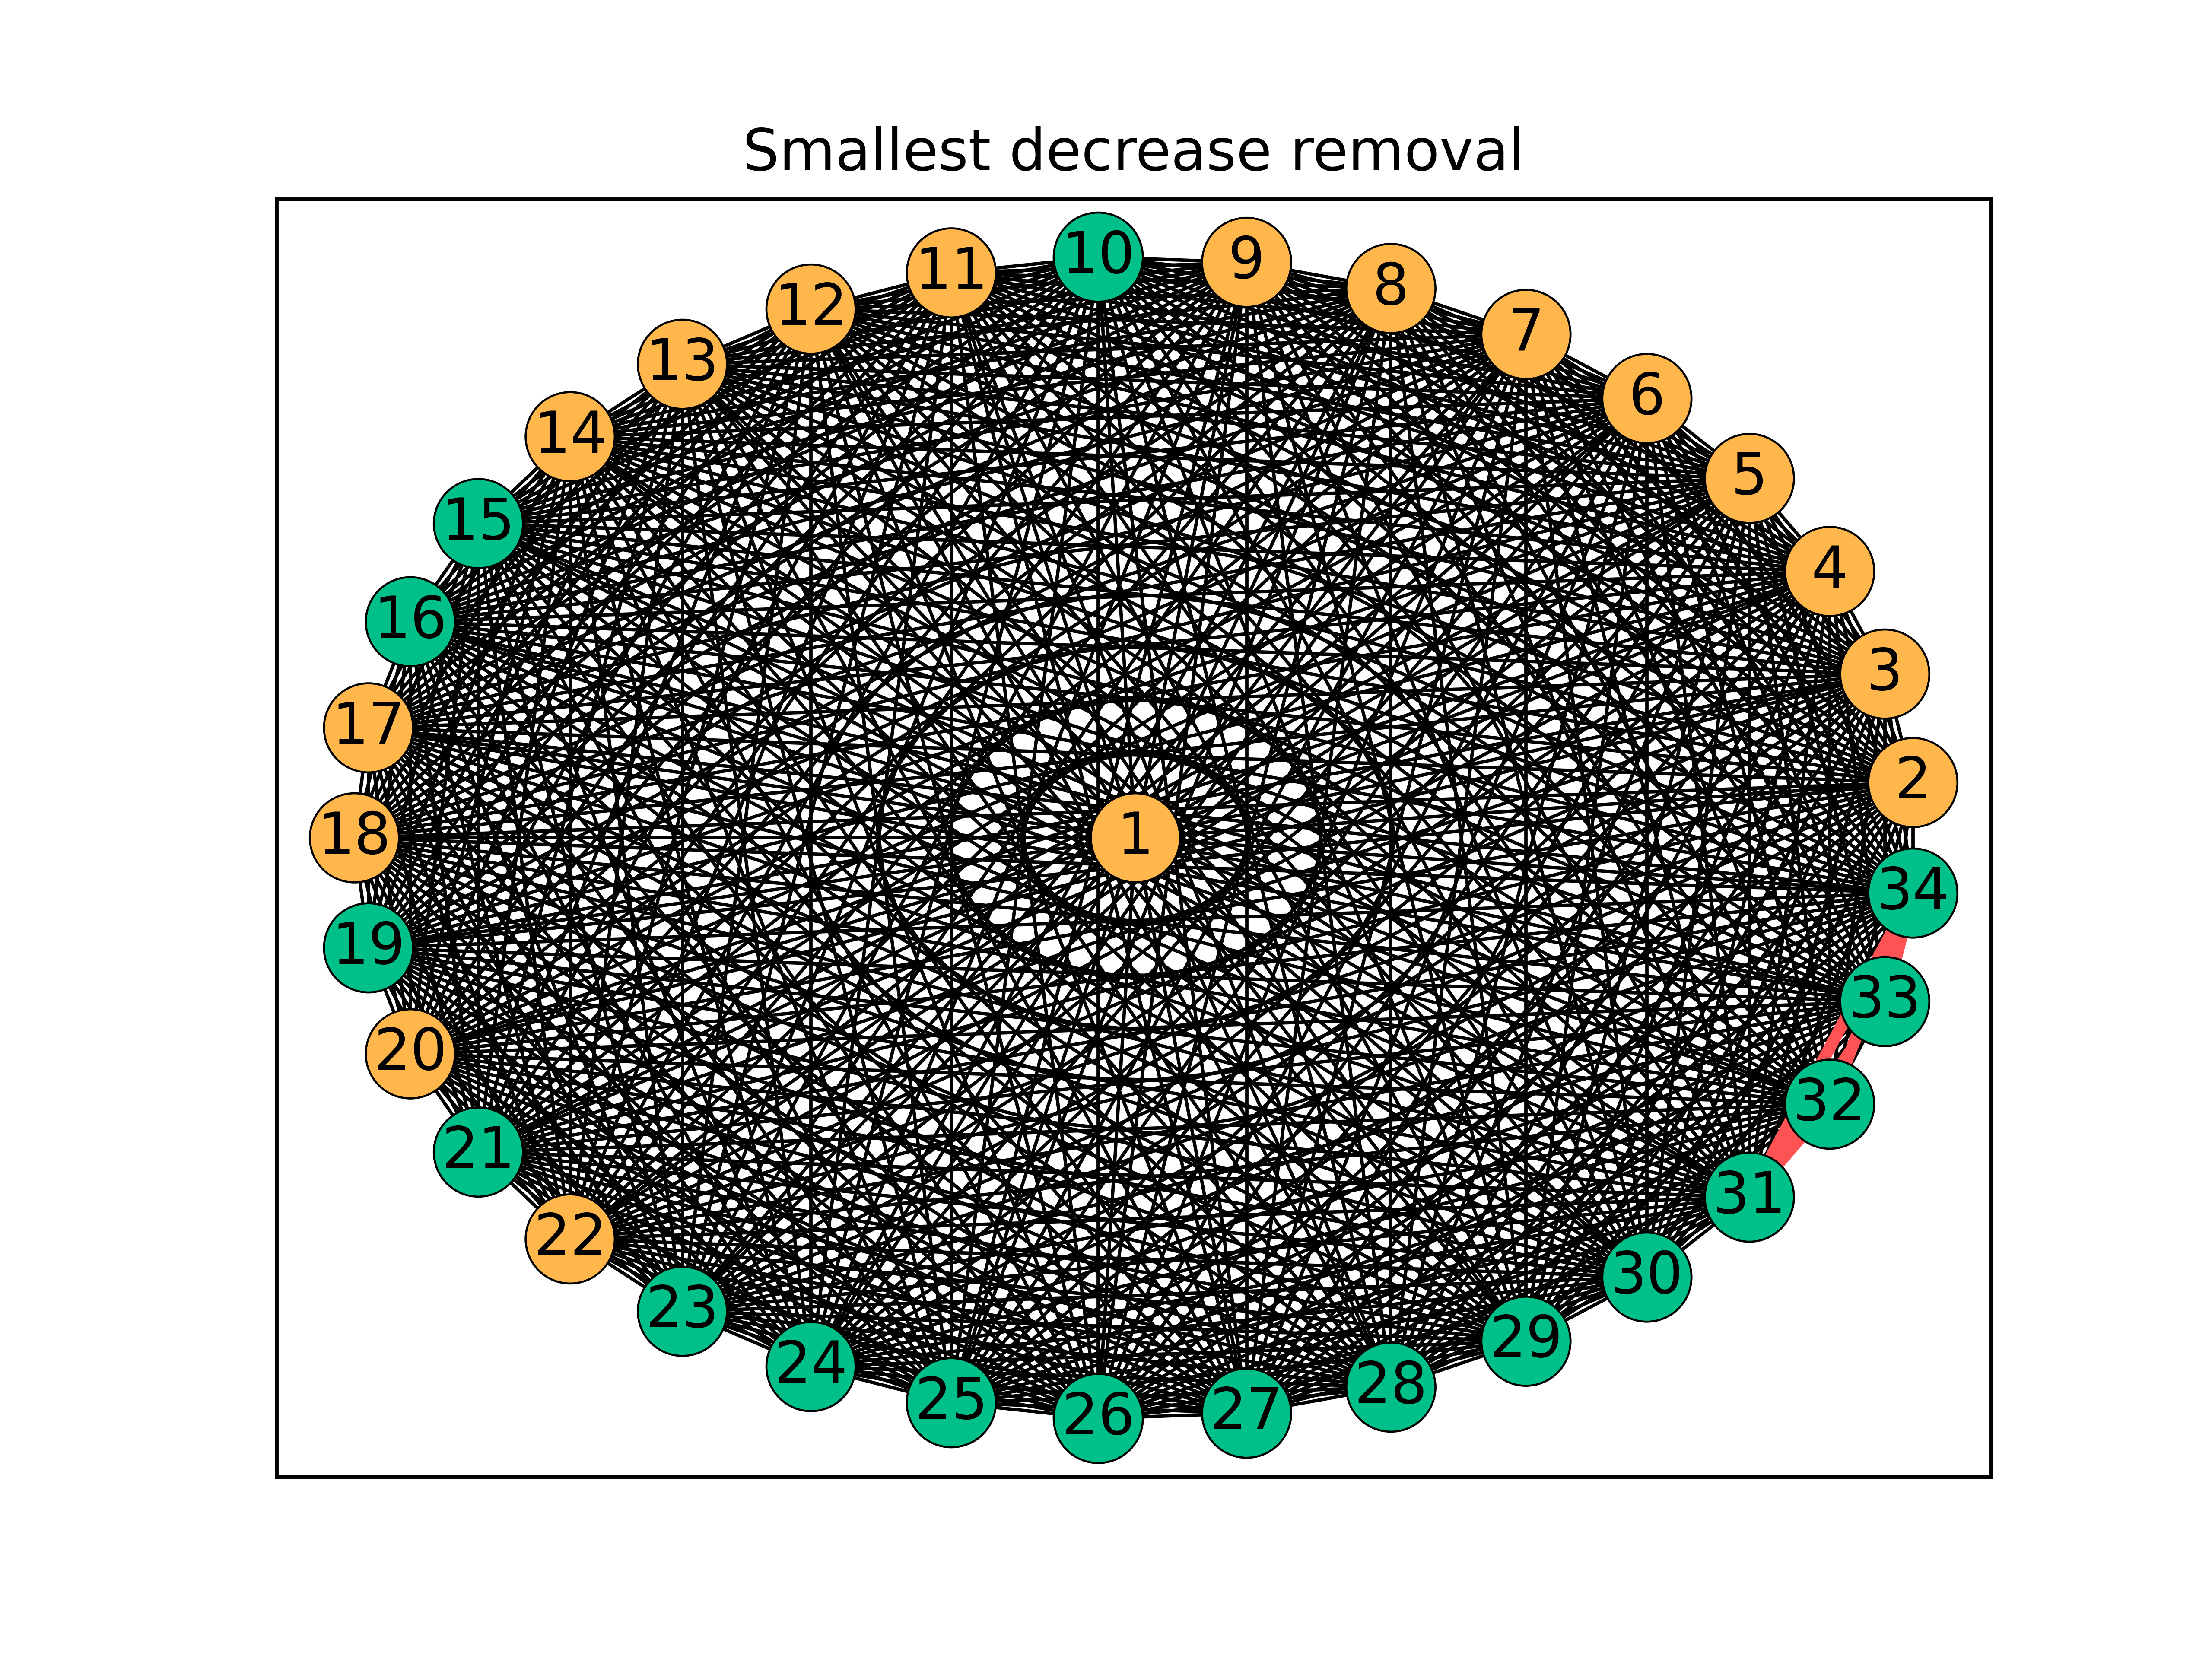
\includegraphics[width=0.70\textwidth]{Figures/smallest.png}
 	\caption{Edge additions}
 	\label{fig:smalest}
\end{figure}



\section{Removing edges and their properties}
\label{sec:properties}
Bellow we examine the removal of edges from the social graph and their result in polarization. We also use the edge betweenness centrality. The edge betweenness centrality is defined as the number of the shortest paths that go through an edge in a graph or network.(add cite Girvan and Newman 2002). 

In the tables following Sign and Addition refer to the multiplication and the addition of the opinions of the nodes that are attached to the specific edge examined.
\\

\begin{table}[!htb]
 \centering
 \caption{Edges with the 5 largest decrease (Karate Dataset)}
 \label{tab:edgesLargest}
 \begin{tabular}{| l || l | l | l | l |}
 \hline
  Edge & Betweeness Centrality & Polarization Decrease & Sign & Addition\\
  \hline
  \hline
  (1, 32) & $0.12725$ & $0.04669$ & - &  0\\
  \hline
  (20, 34) & $0.059384$ & $0.03470$ & - &  0\\
  \hline
  (14, 34) & $0.06782$ & $0.02924$ & - &  0\\
  \hline
  (2, 31) & $0.03228$ & $0.02505$ & - &  0\\
  \hline
  (3, 28) & $0.04119$ & $0.02068$ & - &  0\\
  \hline
 \end{tabular}
 
 \vspace{\floatsep}
 
  \caption{Edges with the 5 smallest decrease (Karate Dataset)}
 \label{tab:edgesLargest}
 \begin{tabular}{| l || l | l | l | l |}
 \hline
  Edge & Betweeness Centrality & Polarization Decrease & Sign & Addition\\
  \hline
  \hline
  (6, 7) & $0.00297$ & $0.0$ & + &  -2\\
  \hline
  (5, 11) & $0.00297$ & $5.55111*10^{-17}$ & + &  -2\\
  \hline
  (4, 8) & $0.00336$ & $3.04869*10^{-7}$ & + &  -2\\
  \hline
  (1, 4) & $0.02049$ & $1.38023*10^{-5}$ & + &  -2\\
  \hline
  (32, 34) & $0.05339$ & $1.61826*10^{-5}$ & - &  +2\\
  \hline
  \hline
 \end{tabular}
 
\end{table}

We can clearly see that there is not a direct association between the edge betweenness centrality and the decrease in polarization. Edge (20,34) has almost the same betweenness centrality with edge (32,34). The one is among the edges that their removal contributes in one of the biggest polarization decrease while the other is among the ones with the smallest. We will examine two more datasets.






